\section{Application of probabilistic catalogs for population studies}
\lb{sec:pop_studies}

\subsection{Number of sources as a function of flux}
\lb{sec:dNdS}


In this section we show how probabilistic catalogs can be used, for instance, for population studies.
One of the most important questions in gamma-ray astronomy is contribution of point sources, 
e.g., AGNs, to the extragalactic gamma-ray flux 
\citep[e.g.,][]{2010ApJ...720..435A, 2011ApJ...738..181M, 2016PhRvL.116o1105A, 2016ApJS..225...18Z, 2016ApJ...826L..31Z, 2016ApJ...832..117L, 2018ApJ...856..106D}:
if most of the extra-galactic emission is explained by point sources, then one can put stringent constraints, 
e.g., on  dark matter annihilation or decay into gamma rays 
\citep{2015ApJ...800L..27A, 2015PhRvD..91l3001D, 2015JCAP...09..008F, 2015PhR...598....1F, 2017ChPhC..41d5104L} or 
on evaporation of primordial black holes \citep{2010PhRvD..81j4019C}.
In particular, it is important to understand the contribution to the population of AGNs from the unassociated sources.
A probabilistic catalog provides an answer to the question: how many sources among the unassociated ones are expected to belong to different classes, such as pulsars or AGNs. 
One can calculate the total expected number of AGNs or pulsars among the unassociated sources, or calculate the contribution as a function of one or more parameters.
In this section we determine the numbers of AGNs and pulsars as a function of their flux.



\begin{figure*}[h]
\center
%\hspace*{-1cm}
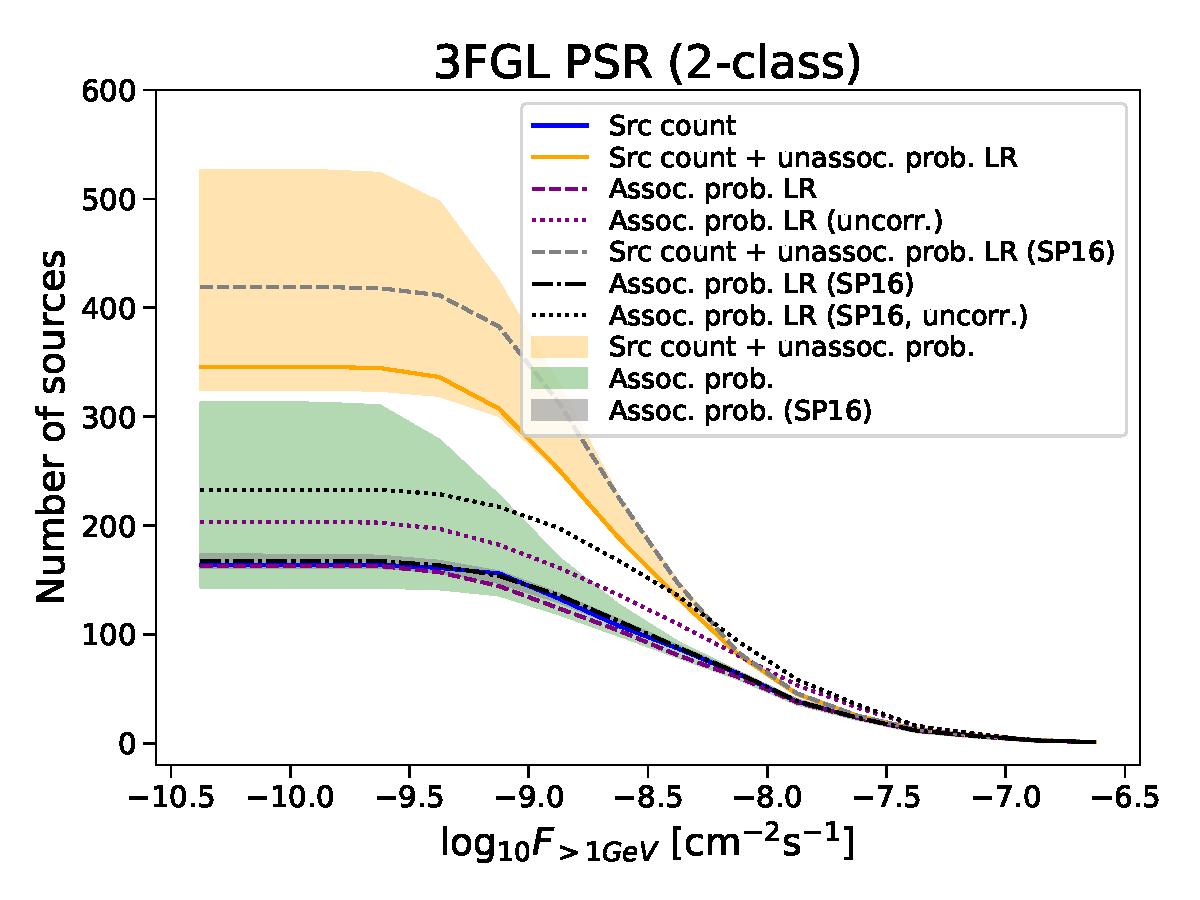
\includegraphics[width=0.45\textwidth]{plots/N_logS_3FGL_PSR_SazP_add_os.pdf}
%\hspace*{-1cm}
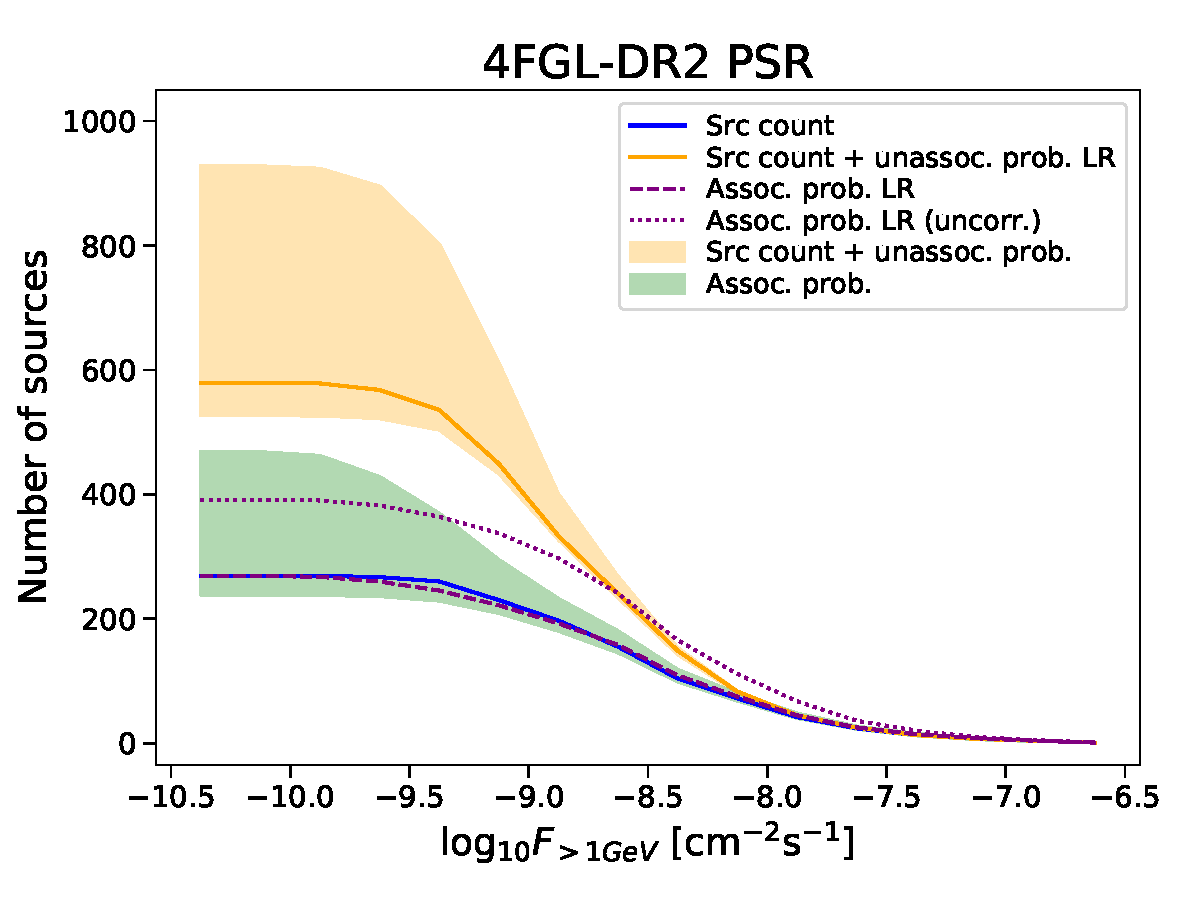
\includegraphics[width=0.45\textwidth]{plots/N_logS_4FGL-DR2_PSR_add_os.pdf} \\
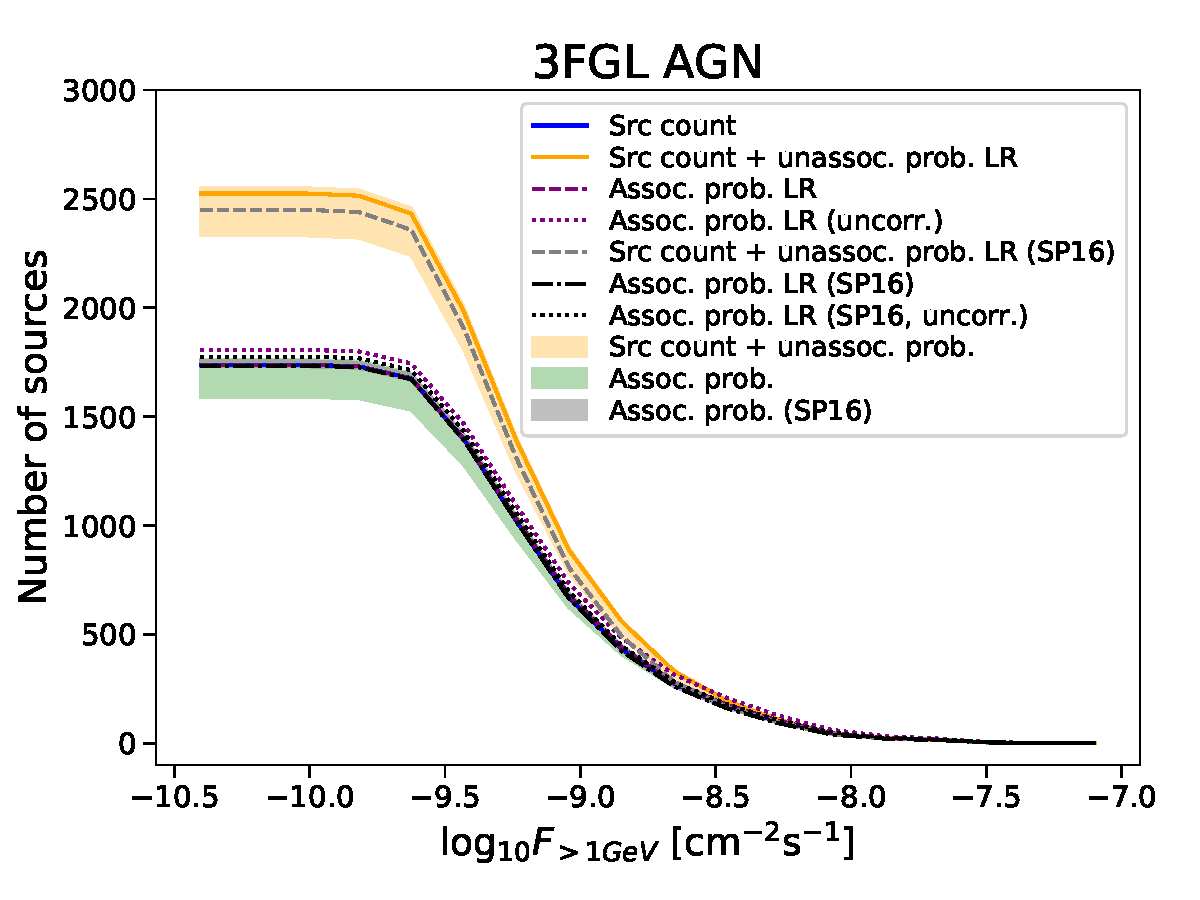
\includegraphics[width=0.45\textwidth]{plots/N_logS_3FGL_AGN_SazP_add_os.pdf}
%\hspace*{-1cm}
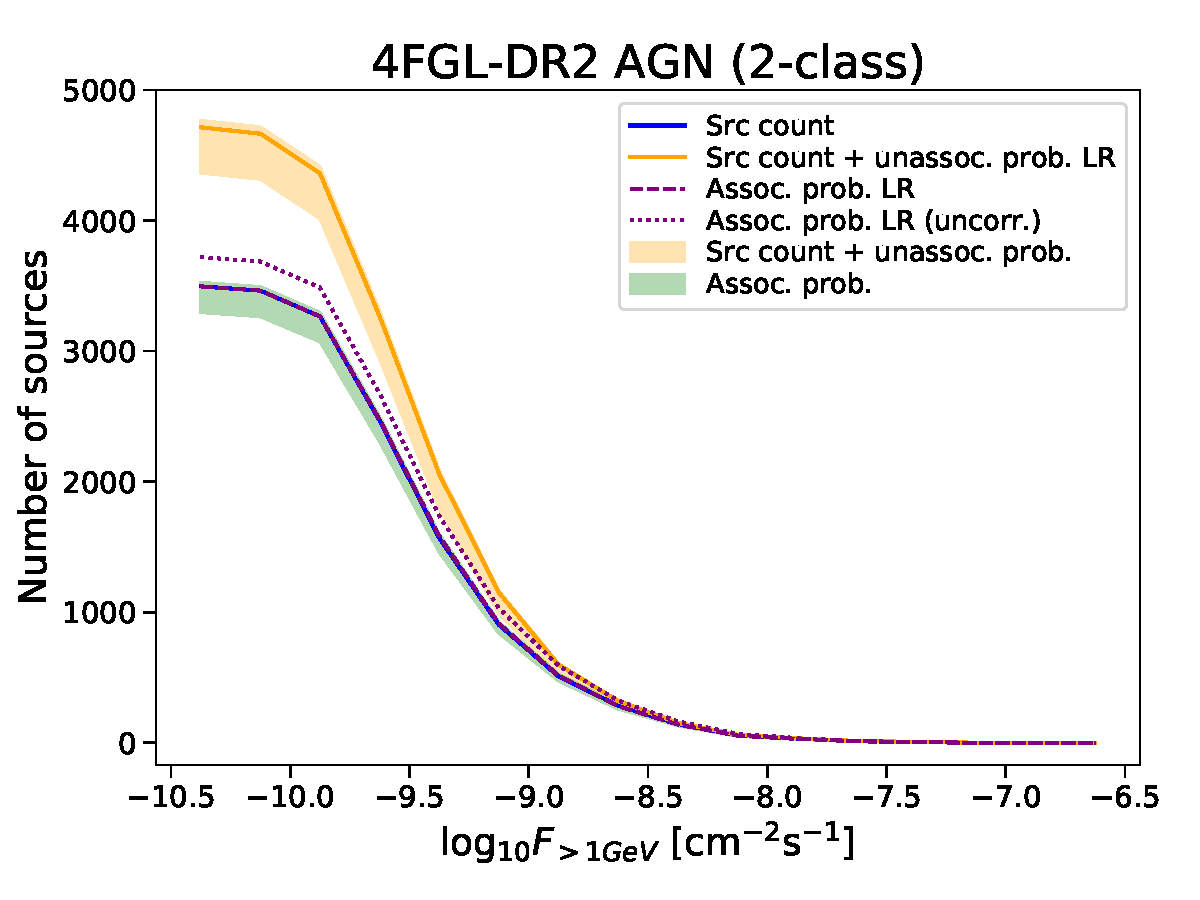
\includegraphics[width=0.45\textwidth]{plots/N_logS_4FGL-DR2_AGN_add_os.pdf}
\caption{Cumulative number of sources as a function of their flux. Green bands show the envelope of the sum of class probabilities for associated sources, while orange bands show the sum of counts of associated sources (blue solid line) plus the sum of probabilities for unassociated sources. The curves with ``SP16'' in the labels are derived from the data in \cite{2016ApJ...820....8S}. For details see Section \ref{sec:dNdS}.}  
\label{fig:logN_logS}
\end{figure*}


\begin{figure}[h]
\center
%\hspace*{-1cm}
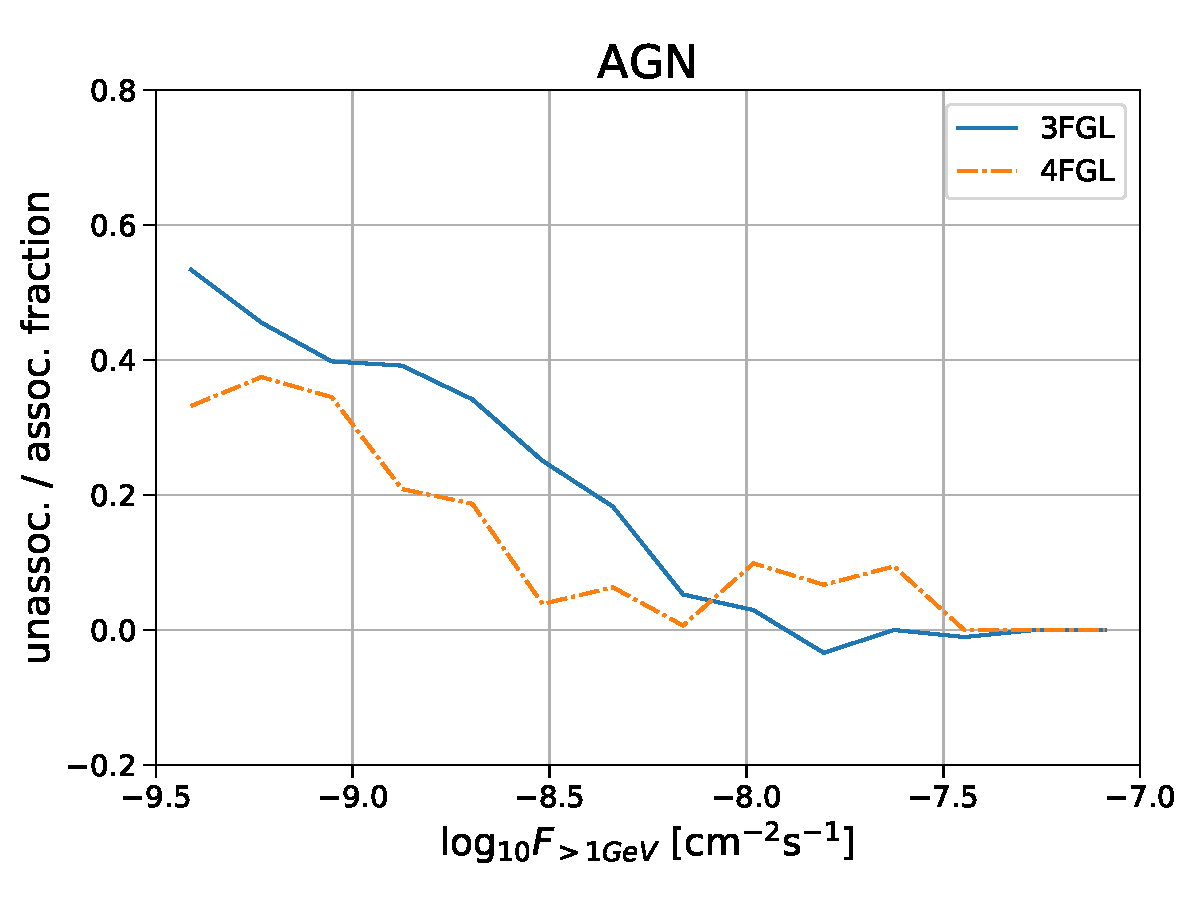
\includegraphics[width=0.45\textwidth]{plots/N_logS_diff_AGN.pdf}
%\hspace*{-1cm}
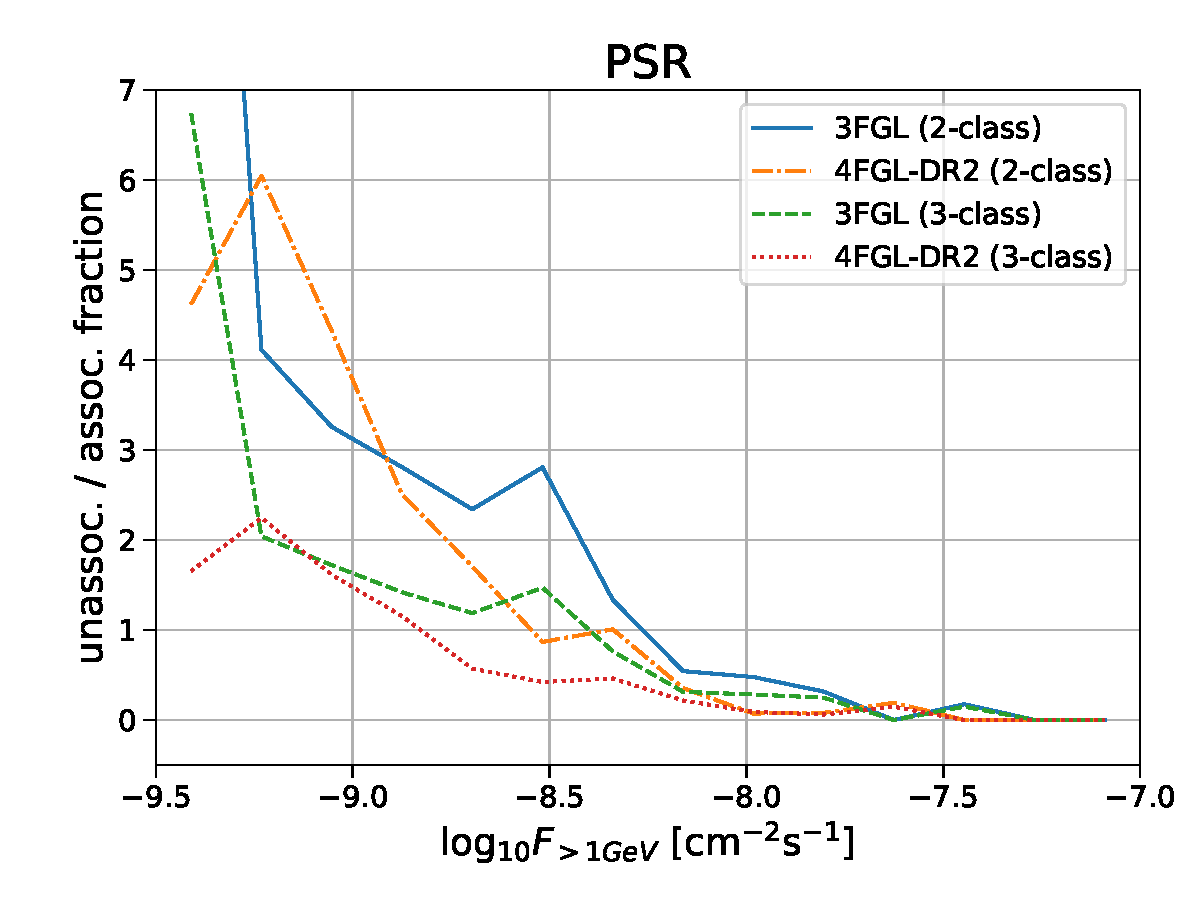
\includegraphics[width=0.45\textwidth]{plots/N_logS_diff_PSR.pdf}
\caption{Ratio of estimated number of AGNs and pulsars among unassociated sources corrected for the presence of other sources (Equation (\ref{eq:unassoc_ev})) to the counts of associated AGNs and pulsars respectively.}  
\label{fig:unass_vs_ass_frac}
\end{figure}




In Figure \ref{fig:logN_logS} we show the cumulative number of AGNs and pulsars with flux above 1 GeV larger than the
value on the x-axis.
Solid blue lines show the actual counts of sources (AGNs or pulsars) in the 3FGL and 4FGL catalogs.
As a consistency check of the method, we calculate the AGN- and PSR-like probabilities for associated sources.
The sum of probabilities (uncorrected for sources other than AGNs and pulsars) for LR algorithm are shown by dotted purple lines.
In order to correct the expected number of AGNs among associated sources for AGN-like probabilities in ``other'' sources, 
we subtract the corresponding AGN-like probabilities in each flux band:

\be
\lb{eq:assoc_ev}
N_{\rm AGN}^{\rm ass}  = \sum_{i \in \rm ass} p^i_{\rm AGN}\,\, - \sum_{i \in \rm ass\,other} p^i_{\rm AGN}.
\ee
The corrected sums of probabilities for LR method are shown by dashed purple lines.
The green bands show the envelope of the sums of corrected probabilities for the eight methods used in this paper.
We see that the counts of associated sources, AGNs and pulsars, are consistent with the expected number of associated sources
calculated from the class probabilities of associated sources.
This conclusion is not very surprising since we used associated sources for training of ML algorithms.
It is important to note that correction for ``other'' sources is important for consistency of the sum of probabilities and the number of associated sources.
We have also compared the sums of probabilities for the 3FGL associated sources in \cite{2016ApJ...820....8S}.
%\footnote{The data is downloaded from \url{https://www.physics.hku.hk/~pablo/pulsarness.html}.} !!! resolve the footnote issue?
The sum of probabilities for associated sources in the LR case uncorrected for ``other'' sources are shown by dotted black line,
while the sums corrected for ``other'' sources are shown by black dash-dotted lines.
The gray band is the envelope of the two methods (LR and RF) used by \cite{2016ApJ...820....8S}.
We see that the sum of probabilities for pulsars overpredicts the pulsar counts in 3FGL, 
while correction for ``other'' sources makes the prediction consistent with the counts of pulsars.

The predictions for the number of AGNs and pulsars among the unassociated sources corrected for ``other'' sources 
added to the 3FGL and 4FGL source counts are shown by solid orange lines (for the LR case).
The orange bands show the corresponding envelopes for the eight ML methods.
We assume that the fractional contribution of other sources is the same for associated and unassociated sources in the different flux bands.
Thus, the correction for the presence of other sources is calculated similarly to the associated sources in Equation \ref{eq:assoc_ev},
but we adjust for the fact that there are fewer unassociated than associated sources, i.e., 
the correction is assumed to be proportionally smaller.
In particular, the number of AGNs among unassociated sources in a flux band $\Delta F$ is estimated as

\be
\lb{eq:unassoc_ev}
N_{\rm AGN}^{\rm unass} = \sum_{i \in \rm unass} p^i_{\rm AGN}\,\, - \sum_{i \in \rm ass\,other} p^i_{\rm AGN} \cdot 
\frac{N_{\rm unass}}{N_{\rm ass}}
\ee
where all probabilities and the numbers of sources are computed for sources with flux inside $\Delta F$.
The first term is the sum of AGN-like probabilities among the unassociated sources,
while the second term is the sum of AGN-like probabilities among associated ``other'' sources rescaled by the total number
of unassociated and associated sources in this flux band.
The expected number of pulsars among the unassociated sources is calculated analogously.
The corresponding sums of associated source counts plus the expected number of sources calculated with LR method of \cite{2016ApJ...820....8S} 
and corrected for other sources are shown by dashed grey lines.


We predict that the expected number of pulsars among the unassociated sources in the 3FGL catalog
is $267 \pm 110$, where the range is the envelop of the sums of probabilities in Equation (\ref{eq:unassoc_ev})
for different ML methods (including oversampling) corrected for other sources among the unassociated sources.
The expected number of pulsars among the unassociated sources in the 4FGL catalog corrected for other sources is 
$386 \pm 179$.
These numbers are larger than the number of associated PSRs without missing values (164 in 3FGL and 237 in 4FGL).
Even at the lower range of expected numbers of pulsars among unassociated sources, there are potentially as many pulsars
as there are associated ones.

We note that according to Table \ref{tab:3FGL_prediction}, the number of unassociated 3FGL sources 
with $p_{\rm PSR} > 0.5$ for all four ML algorithms is 96 (83), while there are 332 (309.5) sources with mixed classification,
uncorrected (corrected) for other sources.
The number of sources with mixed classification (309.5 for 3FGL or 475.5 for 4FGL)
is larger than the range of values for the expected number of pulsars calculated for the sum of probabilities 
(220 for 3FGL or 358 for 4FGL).
It means that the decision which sources are considered to be more likely pulsars is more sensitive to the choice of the ML method
and the probability threshold than the expected number of pulsars calculated from the sum of probabilities.

We also note that the probabilistic classification mostly affects sources with smaller fluxes,
which we illustrate in Figure \ref{fig:unass_vs_ass_frac}, where we show that the ratio of expected number of AGNs and pulsars among 
unassociated sources computed according to Eq. \ref{eq:unassoc_ev} using LR method without oversampling to the number of associated 
sources decreases as the flux increases.
Negative values (e.g., at high fluxes for AGNs) are due to subtraction of probabilities for the ``other'' associated sources.

\subsection{Latitude and longitude profiles}
\lb{sec:lat-lon-profiles}

\begin{figure*}[h]
\center
%\hspace*{-1cm}
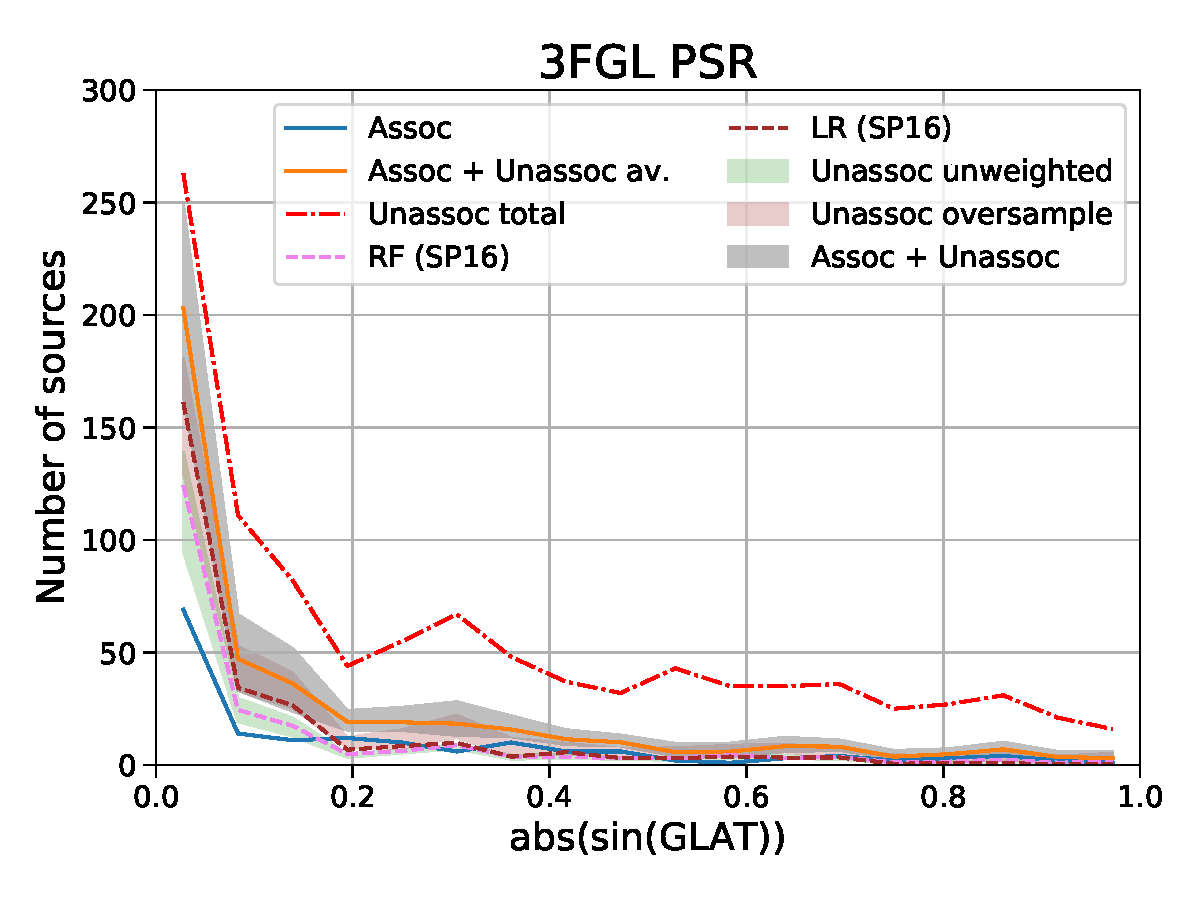
\includegraphics[width=0.45\textwidth]{plots/lat_profile_PSR_3FGL_oversample.pdf}
%\hspace*{-1cm}
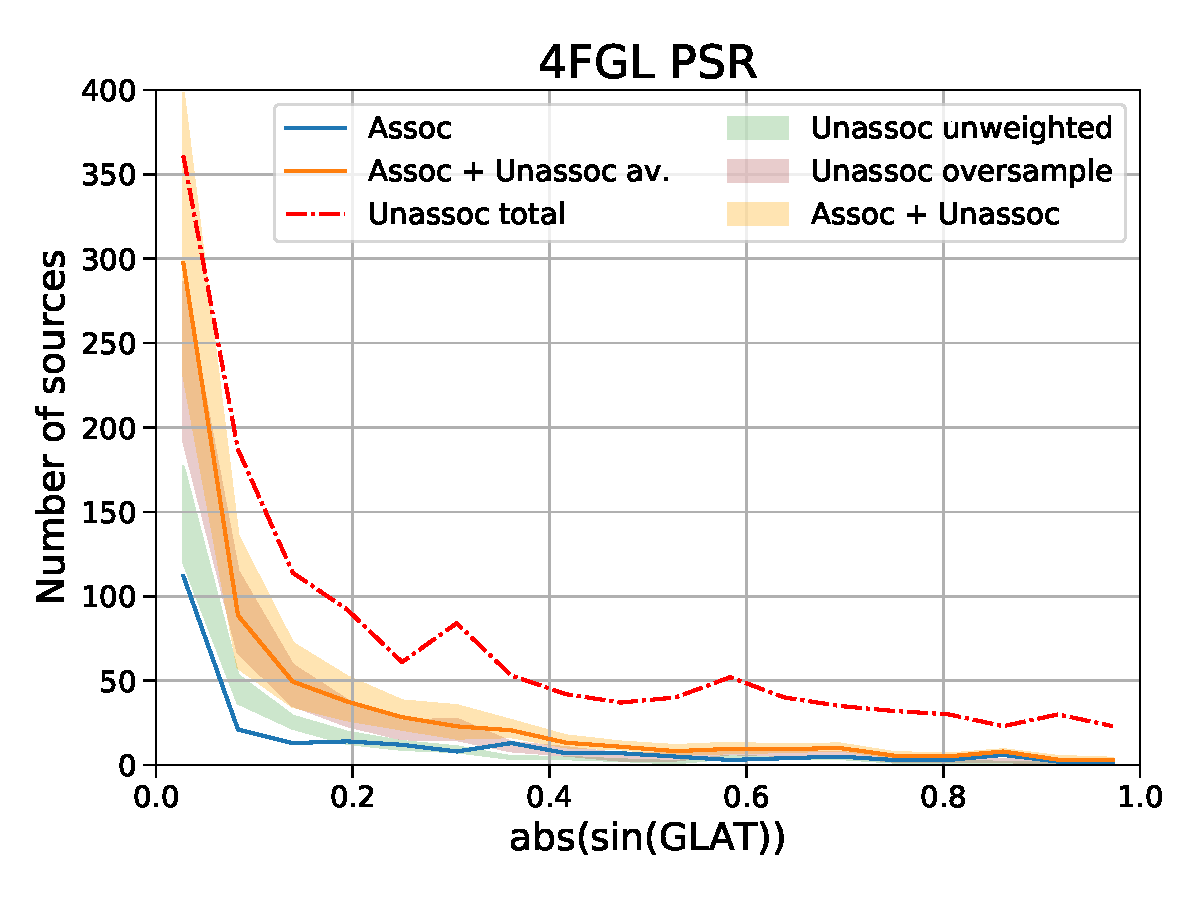
\includegraphics[width=0.45\textwidth]{plots/lat_profile_PSR_4FGL_oversample.pdf} \\
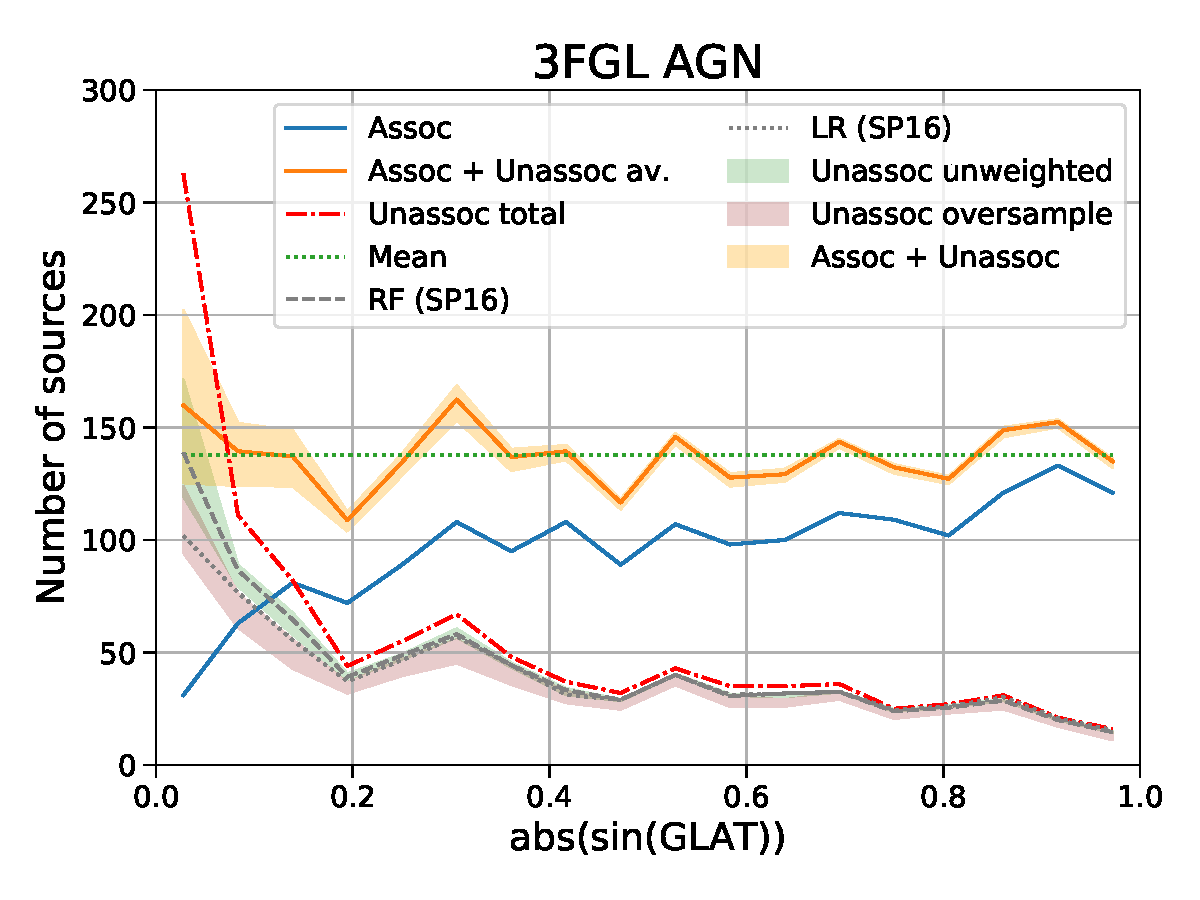
\includegraphics[width=0.45\textwidth]{plots/lat_profile_AGN_3FGL_oversample.pdf}
%\hspace*{-1cm}
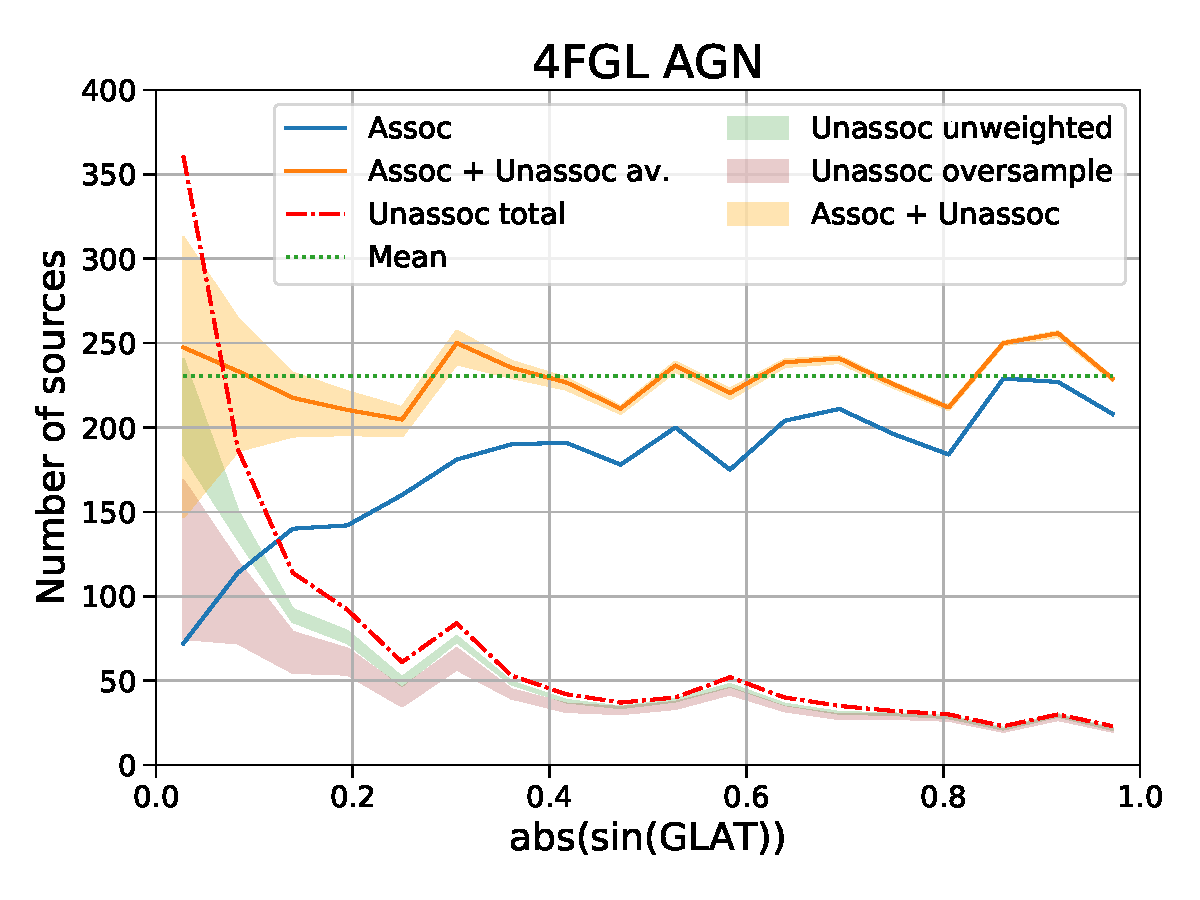
\includegraphics[width=0.45\textwidth]{plots/lat_profile_AGN_4FGL_oversample.pdf}
\caption{Latitude profiles of source counts. Blue solid line -- associated 3FGL and 4FGL sources. Red dash-dotted line -- all unassociated sources. Green (red) band -- envelope of sums of class probabilities for unassociated sources for the four ML algorithms without (with) oversampling. Orange solid line (band) -- average (envelope) of sums of class probabilities for the eight ML methods with and without oversampling added to the source count of associated sources. 
Green dashed line on the AGN plots -- mean of the sum of counts of associated sources and the average of the expectations for counts of unassociated sources (mean of the orange solid line).
Gray dashed (dotted) line -- RF (LR) sums of class probabilities from \cite{2016ApJ...820....8S}.
For details see Section \ref{sec:lat-lon-profiles}. }  
\label{fig:lat_profile}
\end{figure*}



\begin{figure*}[h]
\center
%\hspace*{-1cm}
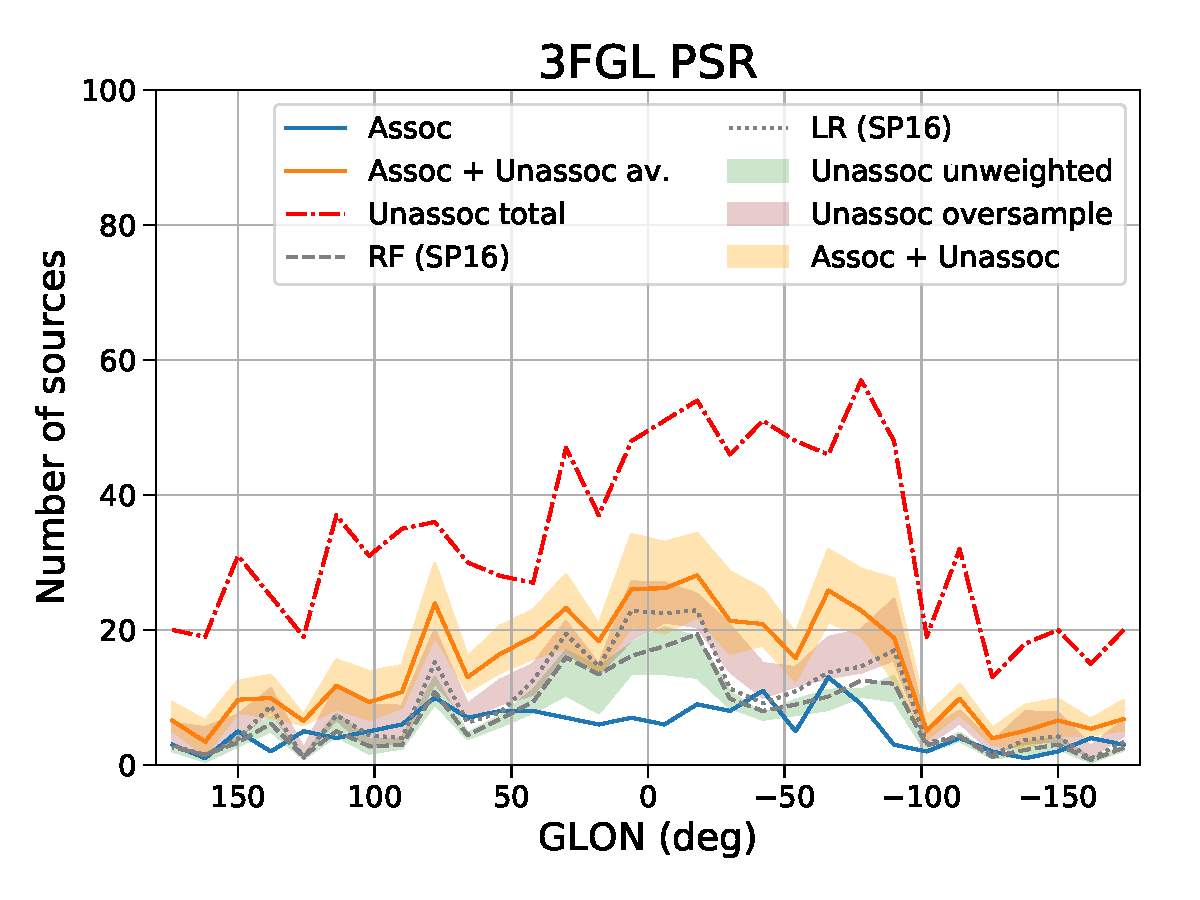
\includegraphics[width=0.45\textwidth]{plots/lon_profile_PSR_3FGL_oversample.pdf}
%\hspace*{-1cm}
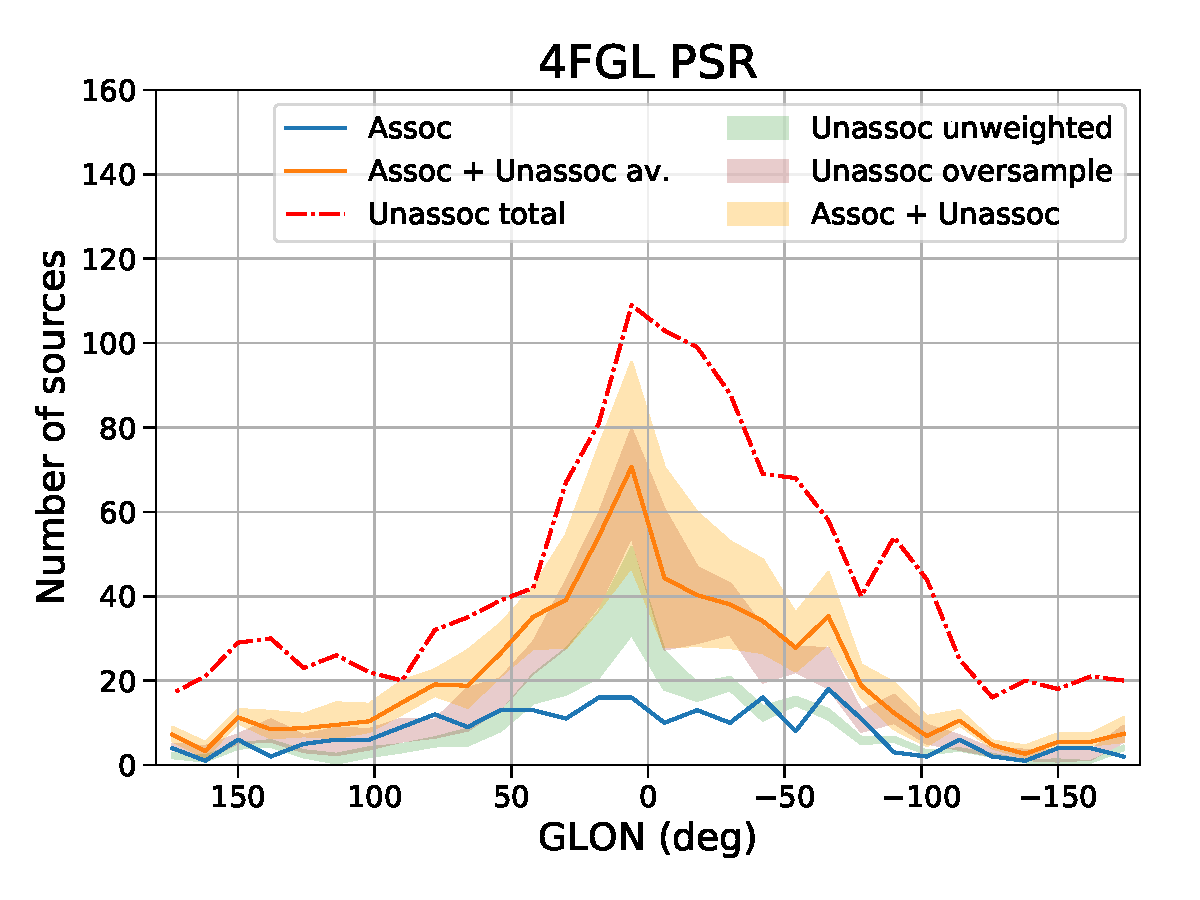
\includegraphics[width=0.45\textwidth]{plots/lon_profile_PSR_4FGL_oversample.pdf} \\
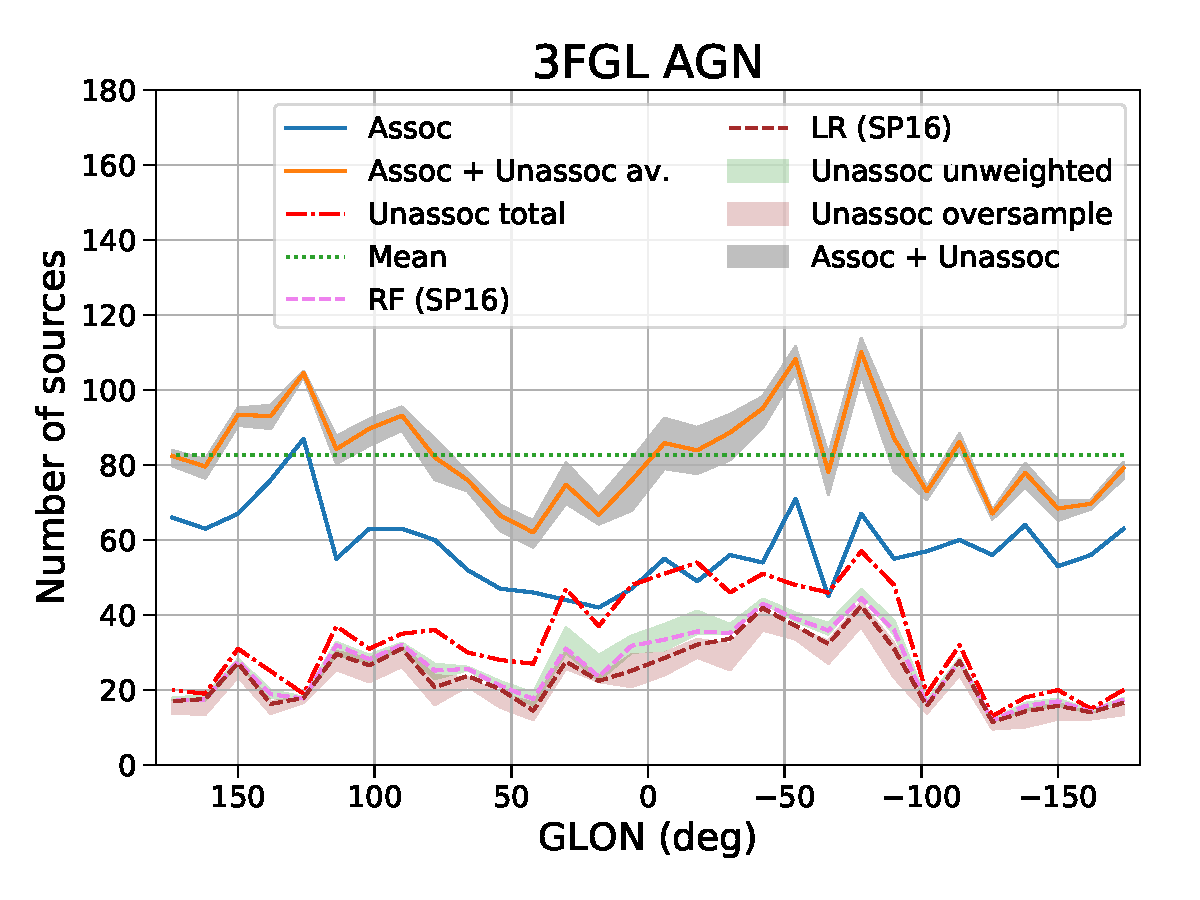
\includegraphics[width=0.45\textwidth]{plots/lon_profile_AGN_3FGL_oversample.pdf}
%\hspace*{-1cm}
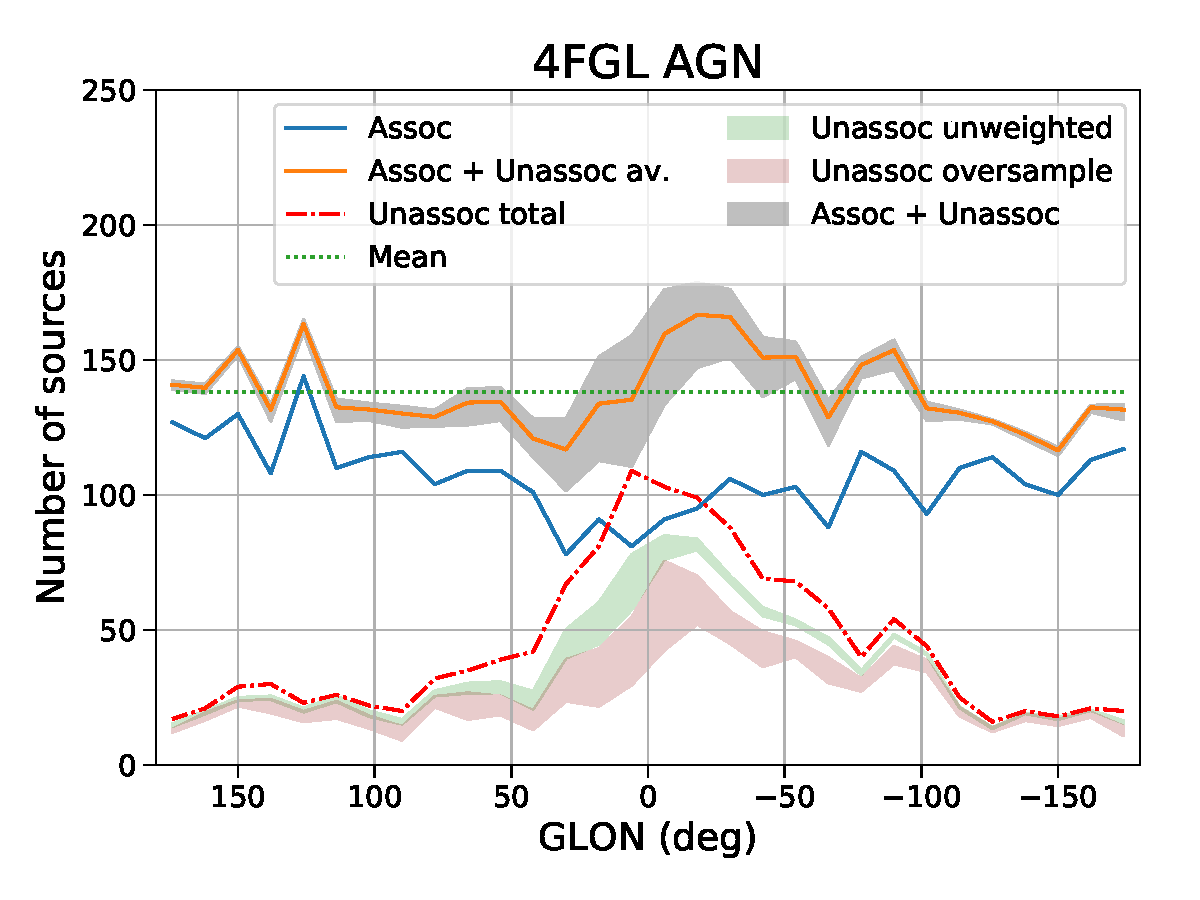
\includegraphics[width=0.45\textwidth]{plots/lon_profile_AGN_4FGL_oversample.pdf}
\caption{Longitude profiles of source counts. For the definition of labels see Figure \ref{fig:lat_profile}.}  
\label{fig:lon_profile}
\end{figure*}


In this section we show Galactic latitude and longitude profiles of the distributions of associated and unassociated sources.
In Figure \ref{fig:lat_profile} we present the source counts as a function of ${\rm abs(sin(GLAT))}$,
where we use 20 bins, i.e., each bin corresponds to a solid angle of $4 \pi / 20$. 
Solid blue lines show counts of associated sources in 3FGL and 4FGL catalogs.
It is interesting to note that the density of associated AGNs is decreasing near the Galactic plane.
The total counts of unassociated sources are shown by red dash-dotted lines.
Green shaded areas show the envelopes of sums of probabilities for AGN- and PSR-like sources for the four 
algorithms without oversampling, while the red shaded areas show the envelope for the four algorithms 
with oversampling.
The classifications of 3FGL sources by \cite{2016ApJ...820....8S} are shown by gray dashed (RF) and dotted (LR) lines.
In this section we do not perform a correction for the presence of other sources among the unassociated ones.
The numbers of unassociated sources classified as AGNs and PSRs grow towards the Galactic plane (GP).
Within $\approx 4^\circ\!\!.5$ from the GP the expected number of PSRs is about the same as the number of AGNs among unassociated sources (the first data point on the left).
At high latitudes, most of unassociated sources are classified as AGNs.
It is interesting to note, that according to Table \ref{tab:feat_imp}, GLAT is one of the least important features for the RF algorithm.
It can be a posteriori explained by the fact that
 the density of AGNs is such that even in the GP the expected number of AGNs is comparable to the expected number of PSRs.

Orange shaded areas show the sum of the source counts and the expected number of sources for the eight methods (both with and without oversampling).
The average among the eight methods added to the counts of associated sources is shown by solid orange line 
(for AGNs we also show the mean of these points by dotted green line).
We find that the number of associated AGNs is decreasing towards the GP, the expected number of AGNs among unassociated sources is increasing towards the GP, but the sum of the two is relatively uniform as a function of Galactic latitude.


In Figure \ref{fig:lon_profile} we show plots analogous to Figure \ref{fig:lat_profile} for Galactic longitudes.
We note that there is a significant increase in the number of unassociated sources in the 4FGL catalog for $|\ell | \lesssim 50^\circ$.
It leads to a large expected number of pulsars among unassociated sources for these longitudes.
The number of associated AGNs is smaller than average for $|\ell | \lesssim 50^\circ$, while the expected number of AGNs among unassociated sources is larger than average for these longitudes.
The sum of the two is relatively uniform, with a possible overprediction of AGNs in the unassociated sources in the 4FGL catalog for \mbox{$-50^\circ < \ell < 0^\circ$}.










